%%%%%%%%%%%%%%%%%%%%%%%%%%%%%%%%%%%%%%%%%%%%%%%%%%%%%%%%%%%%%%%%%%%%%%%%%%%%%%%
%%%%%%%%%%%%%%%%%%%%%%%%%%%%%%%%%%%%%%%%%%%%%%%%%%%%%%%%%%%%%%%%%%%%%%%%%%%%%%%
%%%%  CHAPTER 10 
%%%%%%%%%%%%%%%%%%%%%%%%%%%%%%%%%%%%%%%%%%%%%%%%%%%%%%%%%%%%%%%%%%%%%%%%%%%%%%%
%%%%%%%%%%%%%%%%%%%%%%%%%%%%%%%%%%%%%%%%%%%%%%%%%%%%%%%%%%%%%%%%%%%%%%%%%%%%%%%
\chapter{Experimental procedures}
\label{chap:expprocedures} 


Back in Chapter~\ref{chap:setup-overview} we gave an overview of the
experimental setup and gave some details of the experimental procedure up to
loading the atoms into the optical dipole trap (ODT).    From this point, the
atoms are evaporated down to degeneracy, which leaves them in the dimple trap.
Then we proceed to load the optical lattice where we carry out our experiments.
The operation of the experiment up to the UVMOT step is very robust and very
rarely needs adjustments, other than performing maintenance on the 323~nm laser
system to ensure it has enough output power.   On the other hand, loading
enough atoms into the ODT and making sure that evaporation proceeds properly to
ensure the lowest final temperatures is a critical step which requires much
more attention.   The alignment of the lattice and compensation beams is
extremely sensitive, and is something that needs to be checked every day, and
right before we start taking data.  In fact, we find that our most sensitive
signal (antiferromagnetic (AFM) correlations) only persists for a few hours
after the alignment process, as the beams slightly drift away and get
misaligned.   The process of ramping up the lattice, by slowly rotating the
polarization of the lattice retro beams, is also something that we find
critical for the experiment.  As the polarization is rotated, the power in the
compensation beams is adjusted to ensure that the density distribution of the
atoms does not change much in going from the dimple to the final compensated
lattice. In this chapter, I will give more details about the procedures
outlined above.

\section{Production of a deeply degenerate $^{6}$Li spin mixture in a dimple
potential }

Before we started using the dimple potential as the default starting point of
most of our experiments, we spent significant time optimizing the evaporation
trajectory in the ODT itself.   In the ODT, it is very difficult to
consistently get temperatures below $T/T_{F} \approx 0.10$.   The final
temperature is very sensitive to the final depth of the ODT, which can change
slightly on a daily basis. Drifts in the calibration of the intensity control
loop,  the exact shape of the potential (and therefore the trapping frequencies
which determine the collision rate), or minor changes in alignment and mode
quality of the beams are the principal factors that affect evaporation in the
ODT. 

Despite the sensitivity of the performance of the ODT itself, we found that
adding the dimple potential makes the system much more robust.   We keep the
evaporation trajectory of the ODT the same, and simply ramp up the dimple
potential to a certain depth at the beginning of evaporation, while the ODT is
still deep.  At that point, the dimple ($\sim1.4~\mu$K) is a minor perturbation
on the ODT potential ($\sim300~\mu$K). As the ODT is evaporated away,  the
atoms collect in the dimple, where the trapping frequencies are larger, the
collision rate is increased and evaporation proceeds more efficiently.  We find
that after the ODT is evaporated away, the atoms in the dimple reach the
coldest temperatures that we record,  as low as $T/T_{F}=0.04$.   Depending on
the depth of the dimple, which is set at the beginning, the final number of
atoms can be varied and low temperatures still achieved.  We have verified this
to be the case for atom numbers as high as $N\approx 500,000$ atoms.

\subsection{Optimized trajectory for evaporation in the ODT} 

After loading the atoms from the UVMOT into the ODT the magnetic field is set
to 340~G, where the scattering is $\sim-300a_{0}$.   We keep the depth of the
ODT constant for 1~s, letting the atoms undergo unforced evaporation, and then
we start ramping down the power of the ODT. 

The trajectory for evaporation of the ODT is based on the work by the group of
John Thomas~\cite{OHara2001PRAb,Luo2006}.  It is defined by the following
equations:
\begin{equation}
\text{evap}(t) = 
  \begin{cases}  
   (1-u_{0})     (p_{0}-p_{1})\frac{\tanh \left[\frac{\beta }{\tau
}\frac{p_{1}}{p_{0}-p_{1}} (t-t_{1})\right]}{\tanh\left[\frac{\beta }{\tau
}\frac{p_{1}}{p_{0}-p_{1}}(-t_{1})\right]}+p_{1} +u_{0} 
%
  & \text{if}\ t \leq t_{1} \\ 
   \frac{(1-u_{0})p_{1}}
     {\left(1+\frac{(t-t_{1})}{\tau }\right)^{\beta }} + u_{0}
  &  \text{if}\  t_{1}  < t \leq t_{2} \\
%
   \left(\frac{(1-u_{0})p_{1}}{\left(1+\frac{(t_{2}-t_{1})}{\tau }\right)^{\beta
}}+u_{0}\right)\frac{1}{1+\frac{(t-t_{2})}{\tau_{2}}}
   &   \text{if}\  t_{2}  < t \\
  \end{cases}
\label{eq:evaptraj}
\end{equation}
The first portion is a smoothing ``knee'', to avoid an abrupt start of the
ramps.  The second and third parts use a power law decay with time constants
$\tau$ and $\tau_{2}$.  The initial time constant is appropriate above
degeneracy, and as the gas becomes degenerate ($t\approx t_{2}$) the trajectory
is slowed down ($\tau_{2} > \tau$).  The  trajectory as defined in
Eq.~\ref{eq:evaptraj} has a kink (discontinuous derivative) at $t_{2}$. In
addition to the definition above  we define a time $\delta t$, and for times
$t_{2}
- \delta t/2 < t \leq t_{2} + \delta t/2$ we patch the second and third parts
  of the piece-wise function with a third order polynomial that makes sure the
derivative of the trajectory stays continuous.  The values of the parameters
that we currently use are indicated in Table~\ref{tab:evap}.

\begin{table}
\vspace{0.1em}
\begin{center}
 \begin{tabular}{c|c|c|c|c|c|c|c|c|}
$p_{0}$ &  
$p_{1}$ &  
$t_{1}$ &  
$\tau$  &   
$\beta$ &  
$u_{0}$ &  
$t_{2}$ &  
$\tau_{2}$  &
$\delta t$ 
  \\ \hline
 10.25 & 
 6.5   &
 780~ms  &  
 1400~ms &  
 1.55   & 
 -0.157 & 
 3000~ms  & 
  1000~ms &
 200~ms   
\end{tabular}
\end{center}
\caption{Parameters for the evaporation trajectory.  The scale parameters
($p_{0},\ p_{1},\ u_{0}$) do not have units, and are scaled to the maximum
available ODT power.  We use the convention $p_{\text{max}}=10$ for the maximum
ODT power. The initial power in the trajectory $p_{0}$ is a little bit above
$p_{\text{max}}$ in order to saturate the control AOM at the beginning of the
trajectory. }
\label{tab:evap}
\end{table}

A plot of the trajectory is shown in Fig.~\ref{fig:evap-traj}.  The reader may
have noticed that the equation that defined the trajectory has no physical
units.   We define the maximum stabilized intensity of the ODT as 10, and the
ODT being maximally attenuated as 0 using a scale for $\text{evap}(t)$ that is
linear in the ODT power.   According to our parameters there is a small part of
the trajectory in which we overdrive the intensity stabilization circuitry
($p_{0}>10$), thus getting the maximum power available from the ODT.  The depth
of the ODT depends on the waist of the beams at the crossing point.  It
typically is 300~$\mu$K, but can vary slightly ($\pm50~\mu$K) depending on the
environmental conditions in the lab. 
\begin{figure}
    \centering
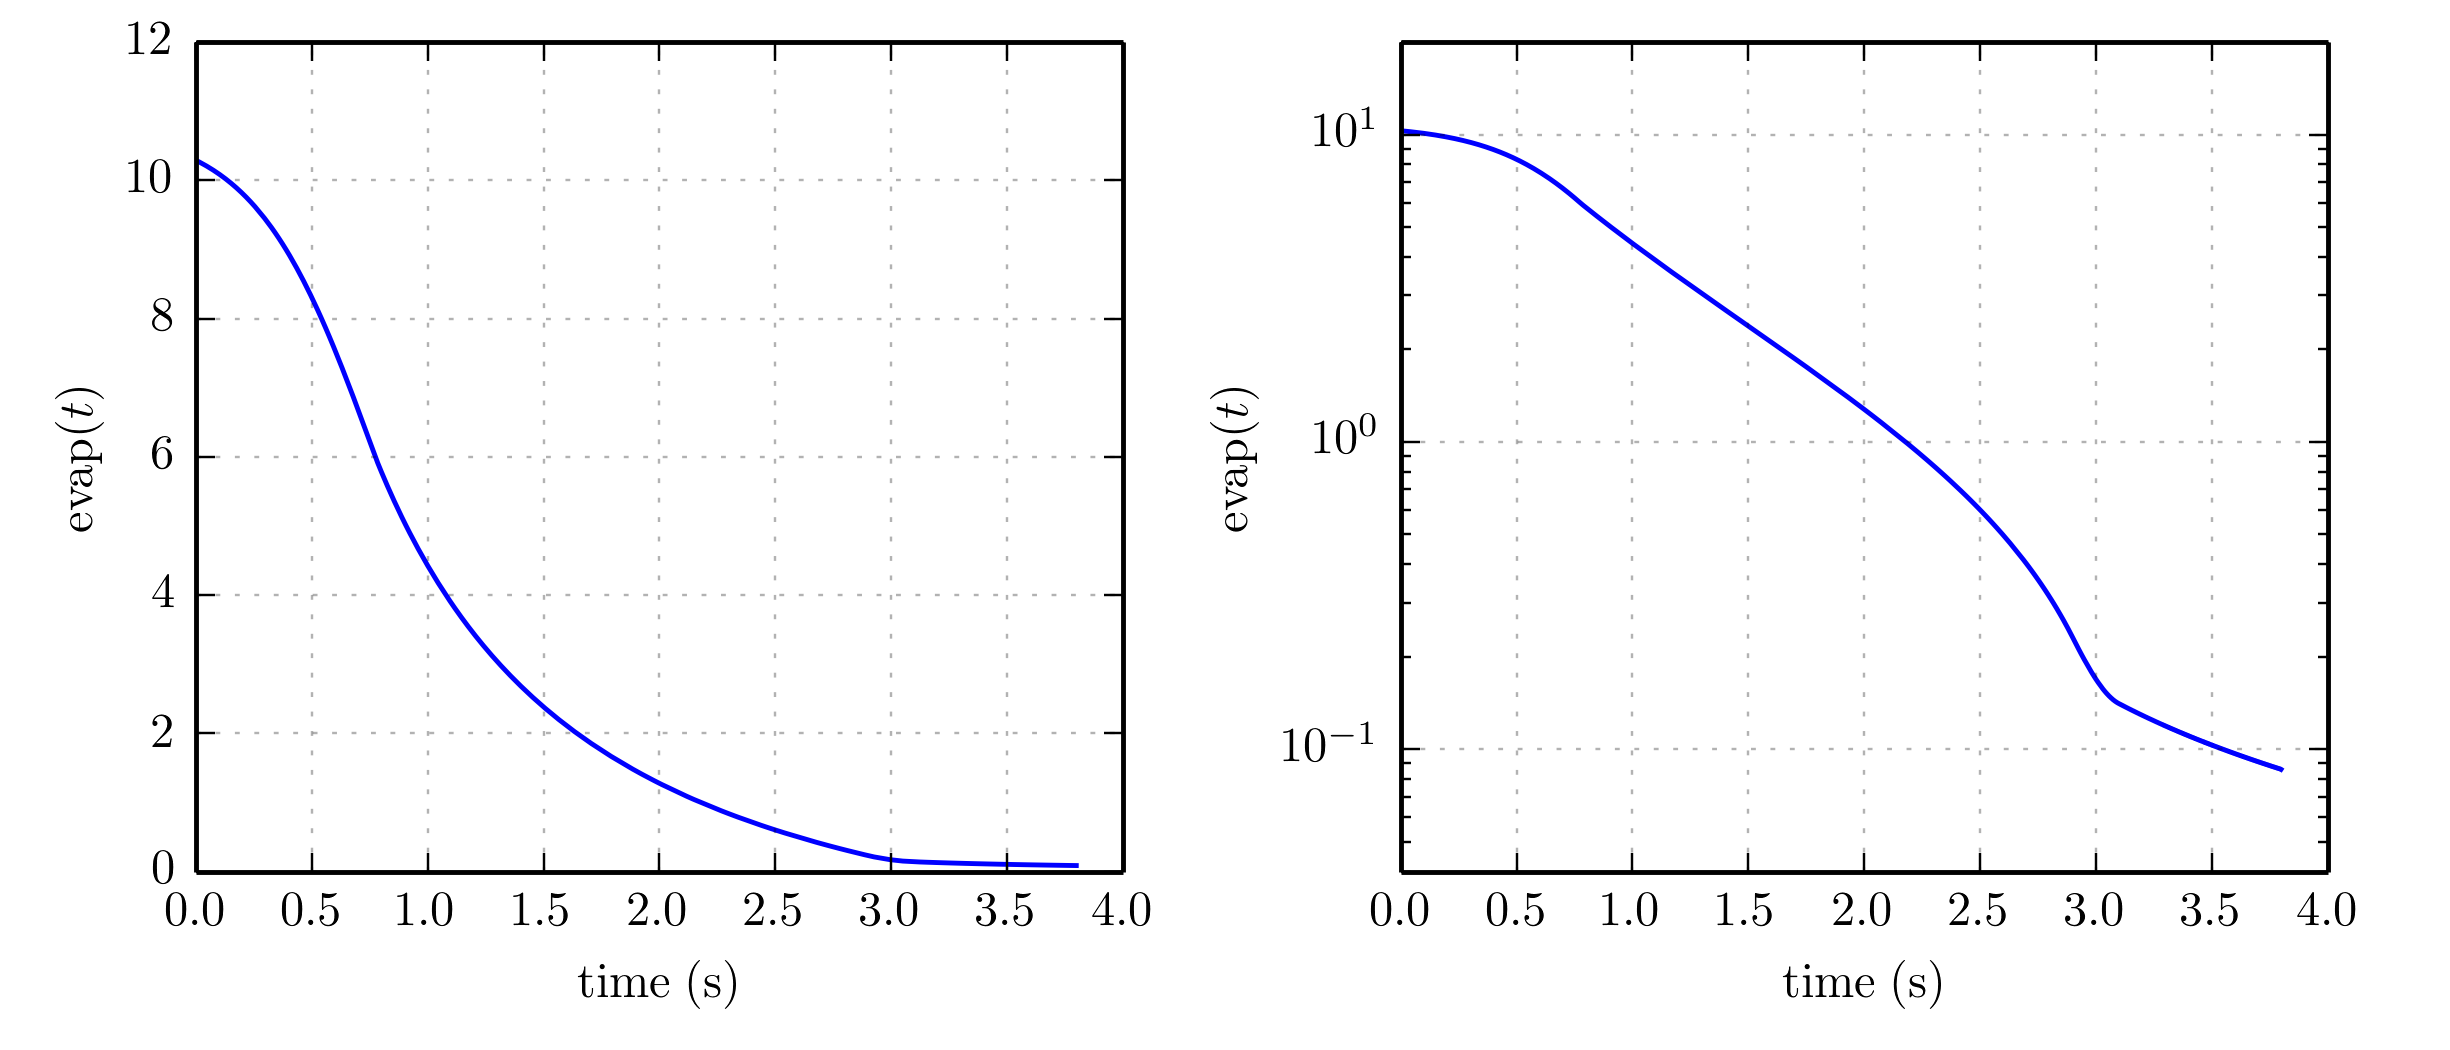
\includegraphics[width=\textwidth]{../figures/evap/evap_traj.png}
\caption{\small Evaporation trajectory defined in Eq.~\ref{eq:evaptraj}. The
parameters used to generate this curve are tabulated in the text. The
evaporation trajectory is shown here up to 3.8 seconds, but the expression in
Eq.~\ref{eq:evaptraj} can be evaluated for longer times. }
\label{fig:evap-traj}
\end{figure}

Along the evaporation trajectory we can measure the temperature of the atoms in
four different ways, which are listed below:
\begin{enumerate}
 \item  From a 2D fit of the column density to a Thomas-Fermi distribution one
can extract $T/T_{F}$ from the fugacity, $e^{\beta\mu}$ (see Eqs.~\ref{eq:ncol}
and \ref{eq:ncolTTF} in Chapter~\ref{chap:fermi-thermometry}).  This only works
for degenerate clouds, $T/T_{F} \lesssim 0.5$.  

\item  From a fit to the azimuthally averaged density distribution, one can
extract $T/T_{F}$ from the fugacity (see Eqs.~\ref{eq:ncol} and
\ref{eq:ncolTTF} in Chapter~\ref{chap:fermi-thermometry}).  This only works for
degenerate cloud, $T/T_{F} \lesssim 0.5$

\item From a fit to the azimuthally averaged density distribution, $T$ can be
extracted from the size of the fit (see Eqs.~\ref{eq:ncolT1} and
\ref{eq:ncolT2} in Chapter~\ref{chap:fermi-thermometry}).  If the trap frequencies are well known,
this can be done using \textit{in-situ} images.  Otherwise a long
time-of-flight (larger than the inverse of the trap frequencies) can be used to
address the momentum distribution directly.   This method works well above and
below degeneracy. 

\item A ballistic expansion measurement can be done, where the size of the
cloud is measured as a function of time-of-flight.  This method only works for
non-degenerate samples with a negative fugacity, $\beta\mu < 0$.  For
degenerate clouds this method can be used as a measure of the Fermi energy. 
\end{enumerate} 

Figure~\ref{fig:evap-data} shows measurements of the temperature using the four
methods outlined above, as a function of time along the evaporation trajectory.
Figure~\ref{fig:evap-data-num} shows the same data in Fig.~\ref{fig:evap-data}
as a function of the atom number remaining in the trap. 
\begin{figure}
    \centering
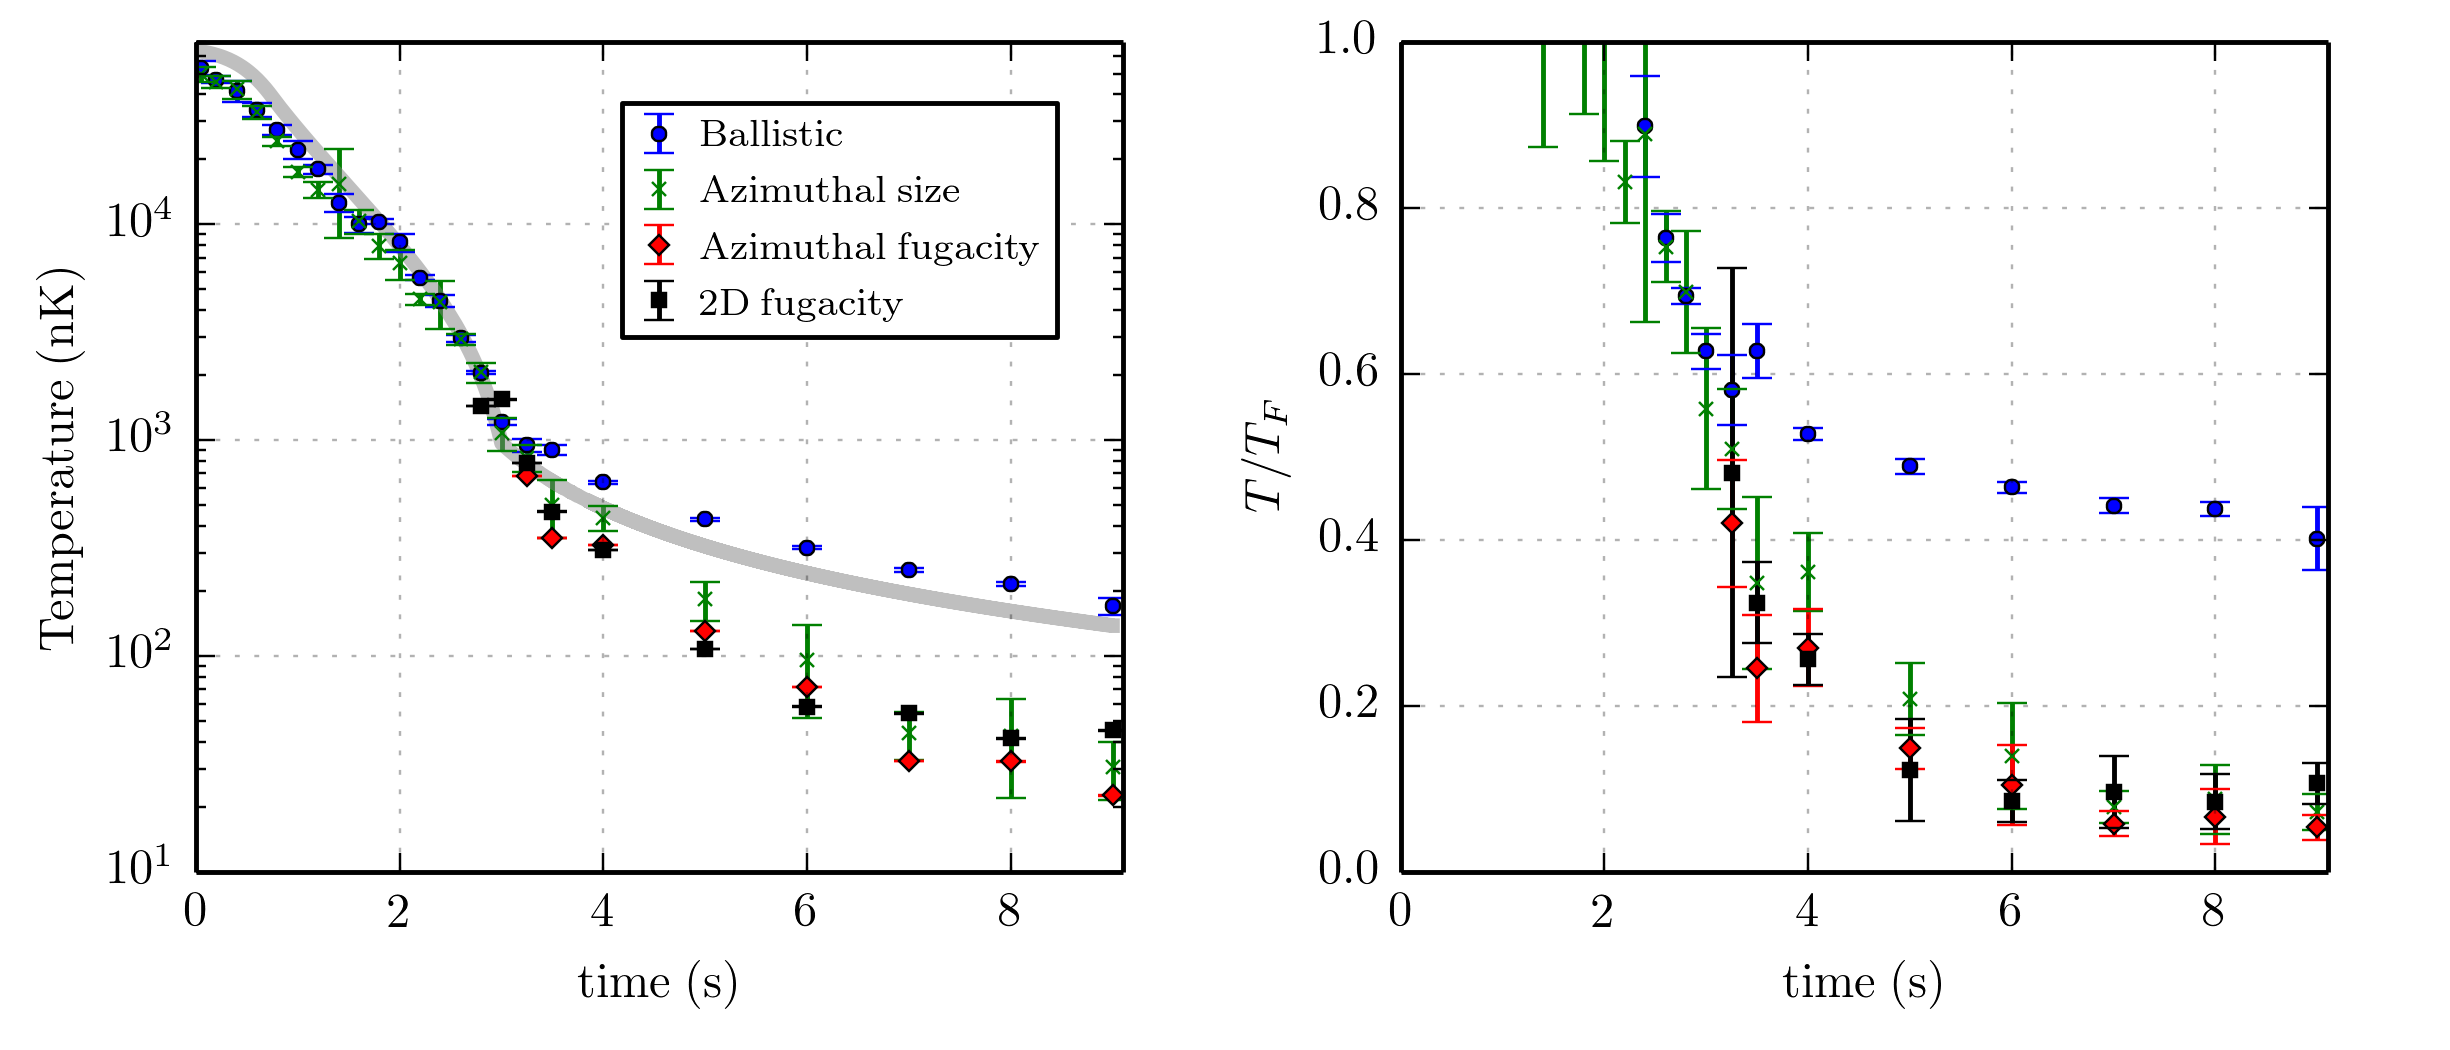
\includegraphics[width=\textwidth]{../figures/evap/evap-data.png}
\caption{\small Temperature in the ODT measured along the evaporation
trajectory defined in Eq.\ref{eq:evaptraj}.  The trap depth divided by a factor
of 5 is shown as a thick gray line. The gas becomes degenerate when the
temperature determined from ballistic expansion deviates from the other
methods.  The Fermi temperature (used to obtain $T$ from measured values of
$T/T_{F}$ is calculated using the calibrated trap frequencies.  The coldest
values are obtained after at least 7~seconds of evaporation and can reach
$T/T_{F}<0.1$ (at that point $T_{F}=564\,$nK).  Note that in the dimple trap we reach
lower temperatures, down to $T/T_{F}\approx 0.04$.  }
\label{fig:evap-data}
\end{figure}
\begin{figure}
    \centering
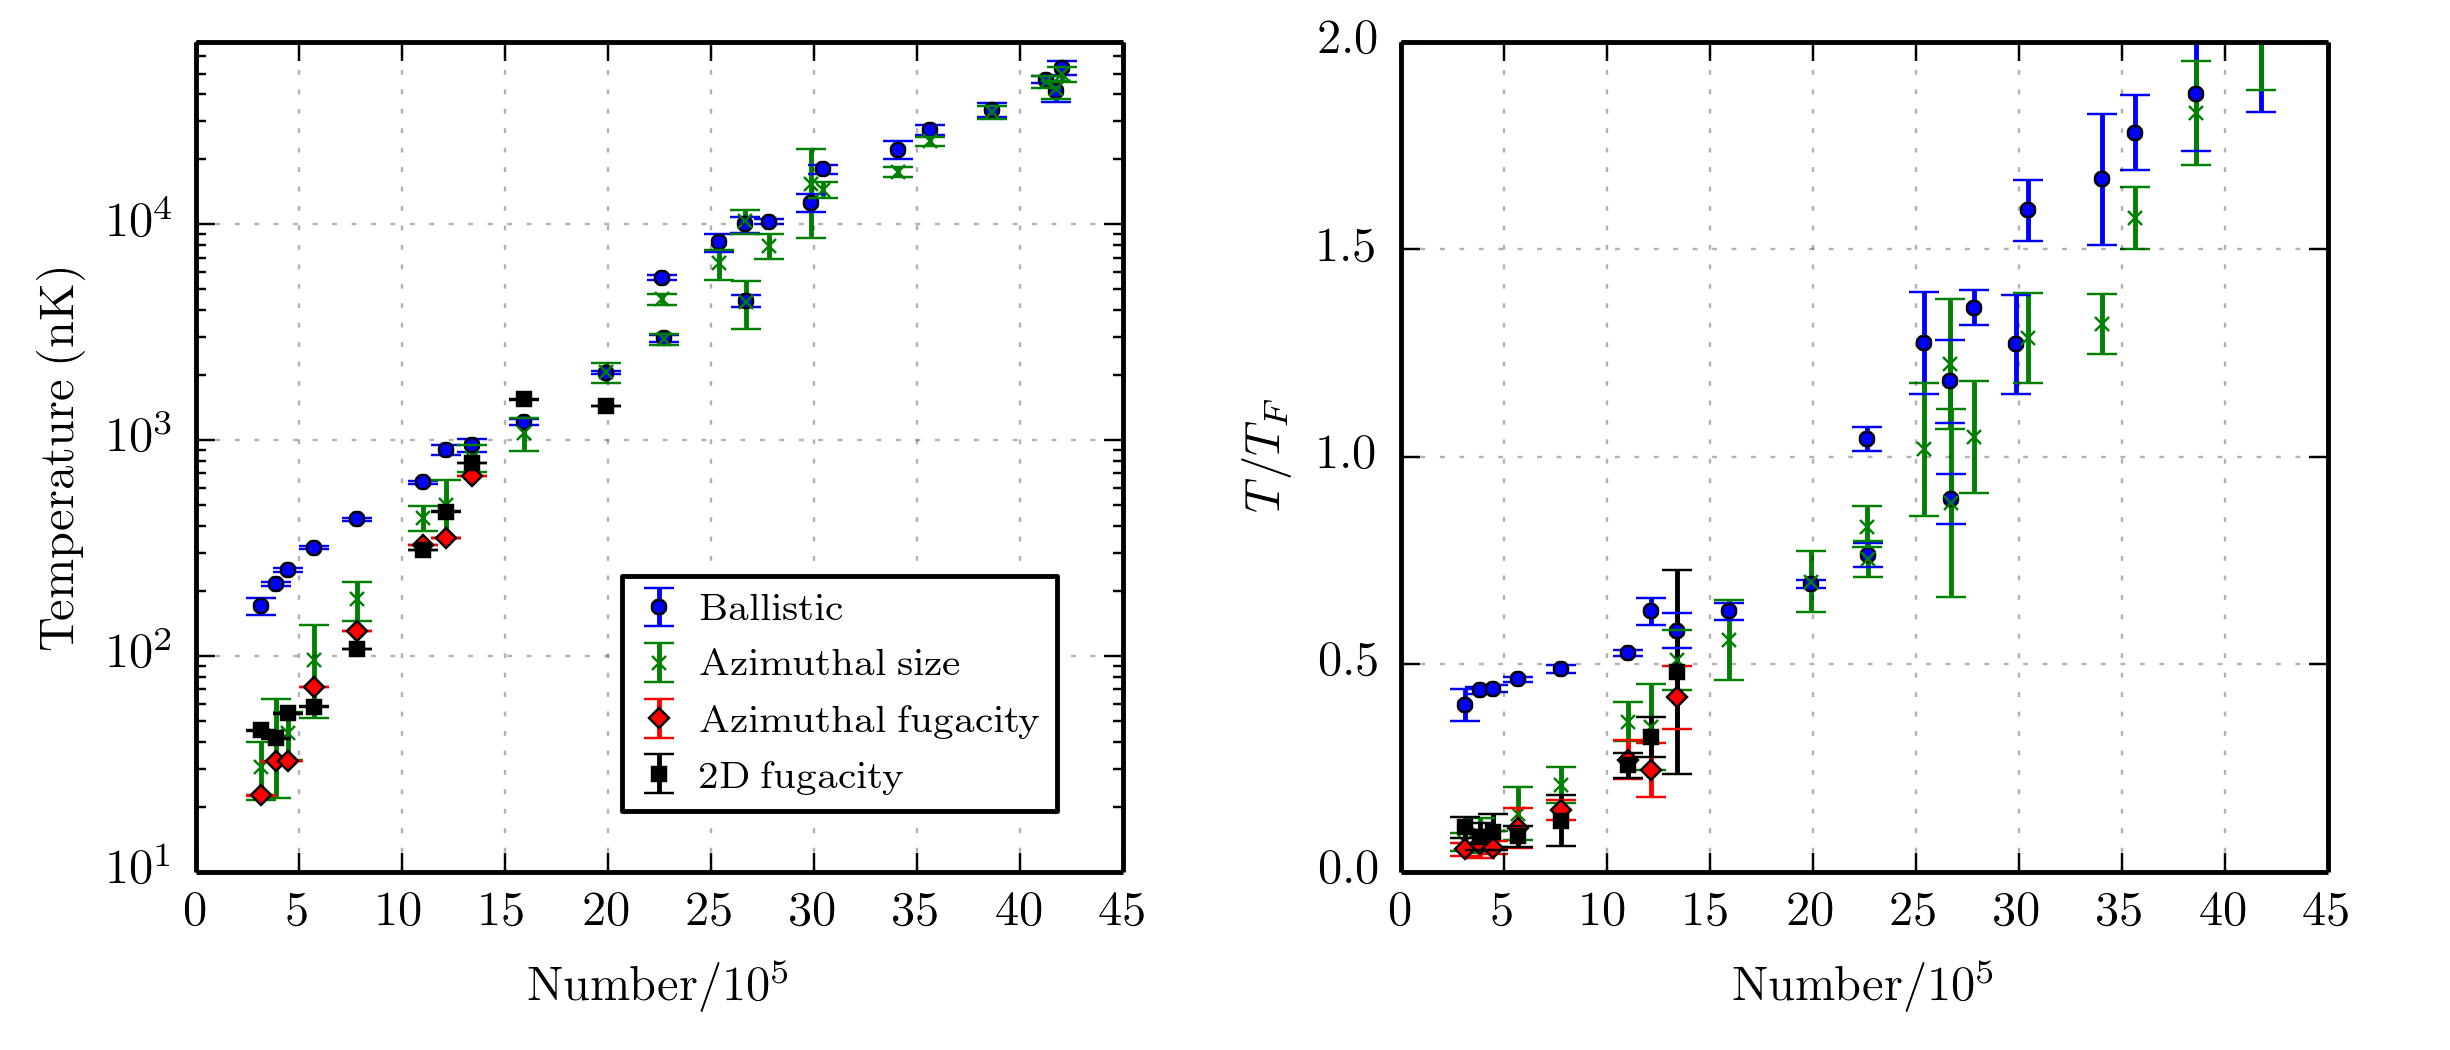
\includegraphics[width=\textwidth]{../figures/evap/evap-data-num.png}
\caption{\small Temperature vs atom number during the evaporation trajectory.}
\label{fig:evap-data-num}
\end{figure}


\subsubsection{Maintenance tips}

Troubleshooting evaporation in the ODT is something we have to do routinely,
below we mention a few points to which one has to pay attention. 

\begin{itemize}
\item The stabilization circuitry for the ODT uses a dual photodiode scheme in
which the feedback transfer function changes abruptly at a point during the
evaporation ramp.  This is discussed in detail in Ernie Yang's Master's
thesis~\cite{ErnieMs}.  The circuit is prone to developing noise if the
parameters to control the gain in the crossover region are not set
appropriately.  One must check the power measured by the stabilization circuit
on the oscilloscope, and make sure that no noise is added on the intensity in
the vicinity of the transfer function kink.  

\item The maximum trap depth of the ODT determines the number of atoms loaded,
which ultimately affects the efficiency of the evaporation trajectory.  To
measure the trap depth, we take the temperature of the atoms after 1~s of
unforced evaporation in the ODT, using a ballistic expansion method.  The idea
is that the scattering length (which is fixed) determines the ratio between the
trap depth and the final temperature after enough time of unforced evaporation.
We usually observe a temperature between 30 and 40~$\mu$K, anything less
indicates that the ODT may not be deep enough.

\item If the ODT is not deep enough there are a few usual suspects.  Number one
is accumulation of dust on the ODT optics.  The prime optic where this happens
is lens labeled $F$ in Fig.~\ref{fig:odtsetup}. Try cleaning that lens first
and then go after any optic that faces upwards.  The proper
crossing of the two ODT passes is also critical, as is the efficiency of the
AOM that controls the ODT intensity. 

\end{itemize} 

\subsection{Modifications to the trajectory for evaporating into the dimple}

When evaporating the atoms from the ODT into the dimple trap we make a few
simple changes to the evaporation trajectory.  The magnetic field is changed
3~seconds into the evaporation, going from 340~G ($-300a_{0}$) to 595~G
($+326a_{0}$).  This is done so that we finish up preparing the sample in the
vicinity of the magnetic field necessary to realize a Hubbard model with
repulsive interactions.   During the 1~s of unforced evaporation, right after
loading the atoms from the ODT, the dimple trap is slowly ramped up to the
desired depth.  This depth is varied to control the number of atoms in the
sample.  Finally, after evaporating the ODT  for 5.5~s (using the trajectory
defined in Eq.~\ref{eq:evaptraj}), we turn it completely off using a smooth
(hyperbolic tangent) turn-off ramp with a time constant of 80~ms.  The ramps
used for this procedure are shown in Fig.~\ref{fig:dimple-evap} 
\begin{figure}
    \centering
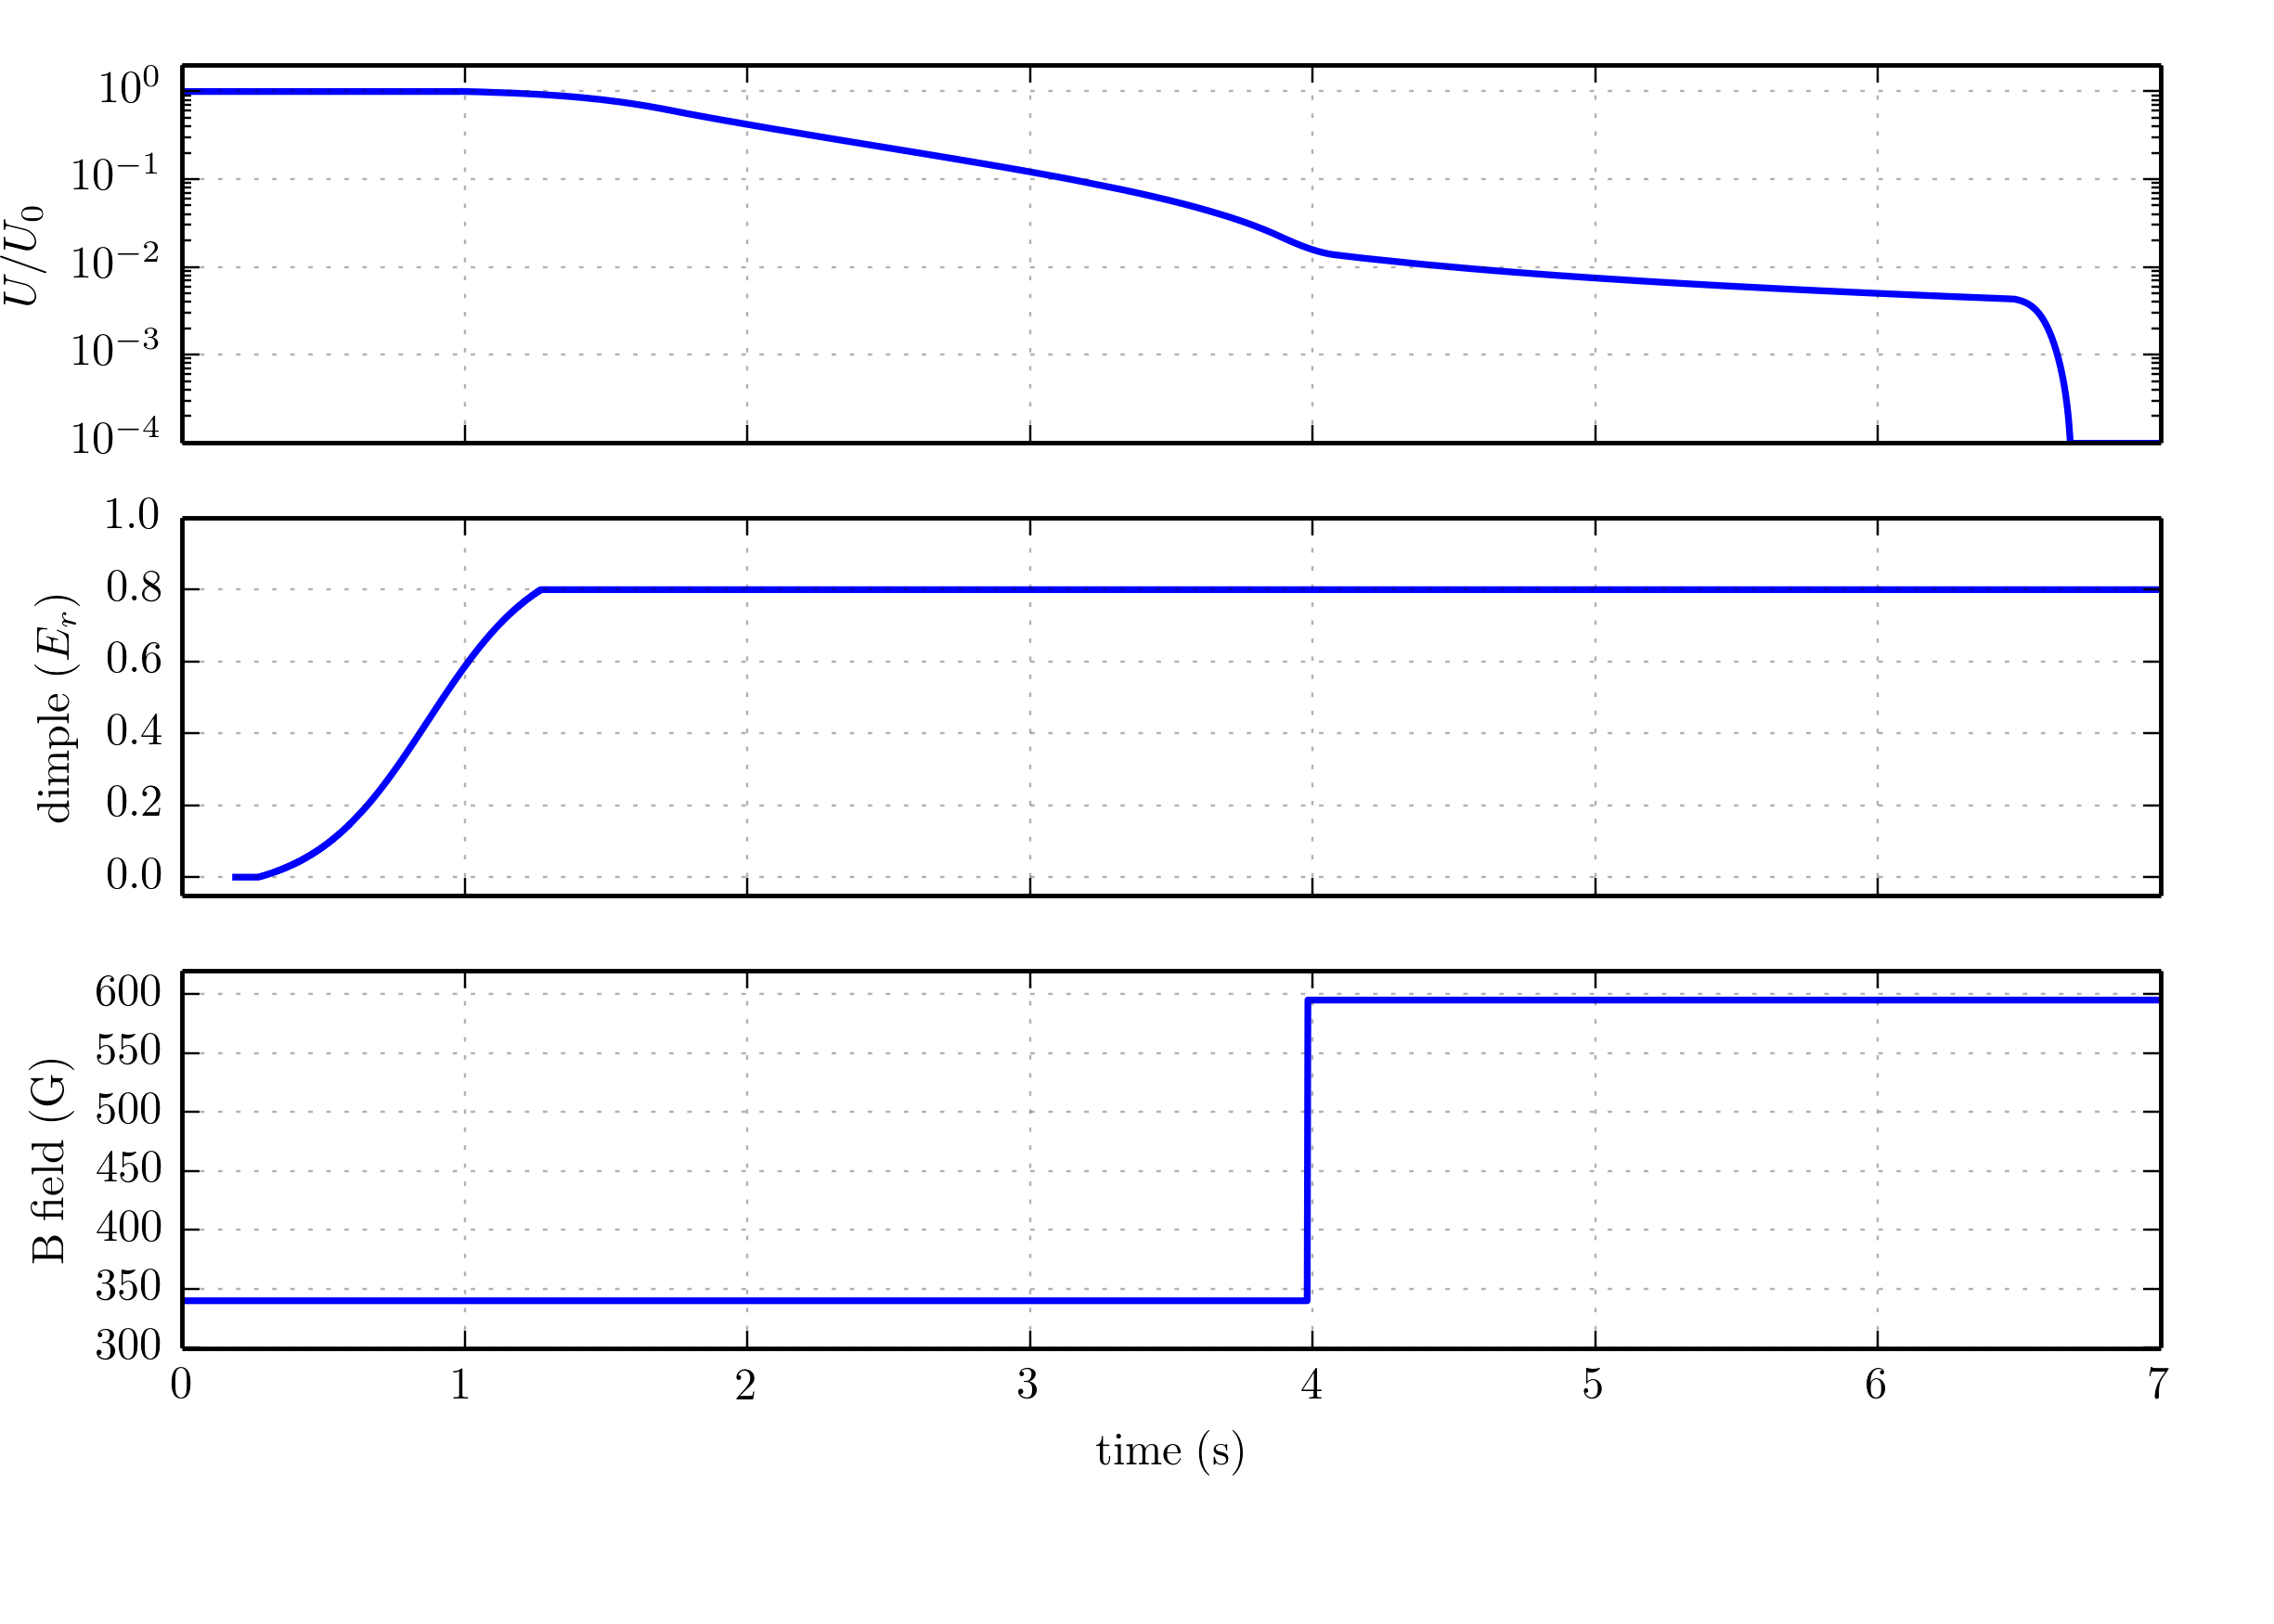
\includegraphics[width=\textwidth]{../figures/evap/dimple_traj.png}
\caption{\small Ramps for evaporating atoms into the dimple trap.  The top plot
shows the relative depth of the ODT. There is 1~s of unforced evaporation
before initiating the 5.5~s of forced evaporation (according to the trajectory
in Eq.~\ref{eq:evaptraj}). The central plot shows the dimple trap depth per
beam, which is turned on at the very beginning during the unforced evaporation.
The bottom plot shows the magnetic field.  At $t=7~$s a degenerate cloud at
$T/T_{F} \approx 0.04$ is produced in the dimple trap. }
\label{fig:dimple-evap}
\end{figure}
 
\subsubsection{$T/T_{F}$ measurement} 

After evaporation into the dimple trap we measure $T/T_{F}$ by imaging the
atoms after 0.5~ms of time-of-flight.   The distribution is allowed to expand
so that we effectively gain some resolution, necessary to capture the details
of the tail of the distribution, to which the temperature fit is most
sensitive.   An example of a cold cloud released from the dimple is shown in
Fig.~\ref{fig:cold}.  
\begin{figure}
    \centering
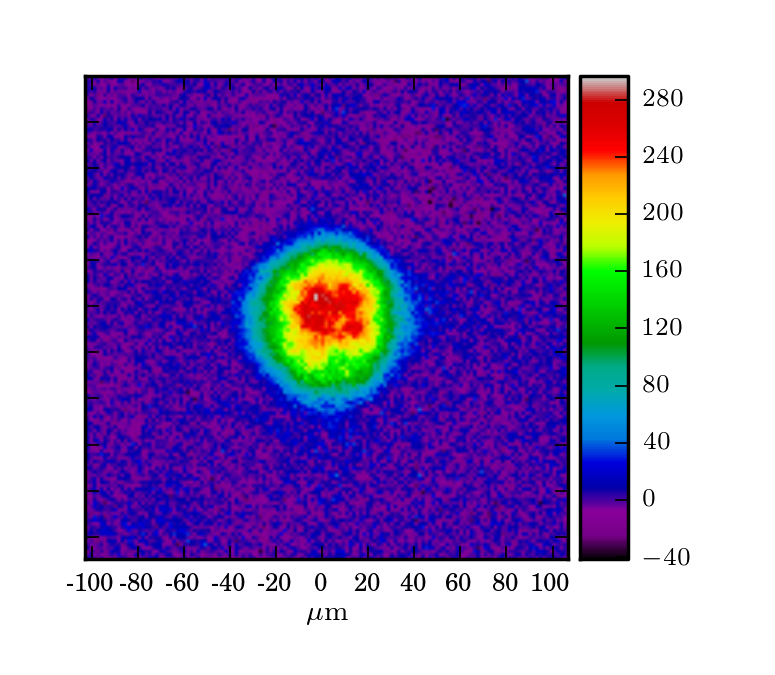
\includegraphics[width=0.49\textwidth]{../figures/evap/cold_coldens.png} ~
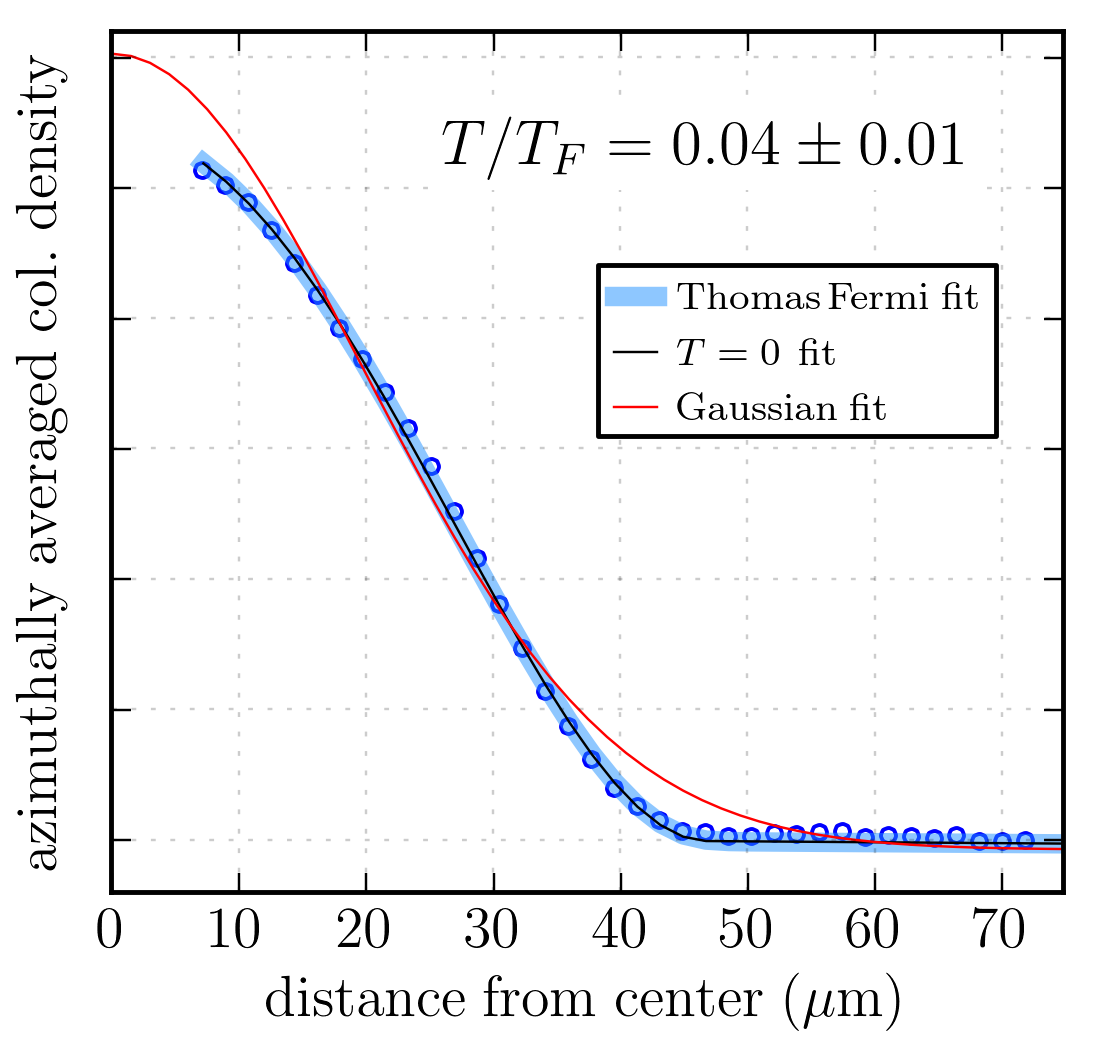
\includegraphics[width=0.42\textwidth]{../figures/evap/cold_az.png}
\caption{\small (Left) Average of the column density for 6 shots.  Images taken
after 0.5~ms TOF. (Right) Azimuthal average of the column density for a single
shot, along with curves showing different fits to the distribution. The
azimuthal average at small radii tends to have larger noise, so we exclude the
first few data points from the fit.  }
\label{fig:cold}
\end{figure}
We determine the temperature from fits to the column density distribution and
also fits to the azimuthal average of the column density distribution.  The
fitting procedures were introduced in Chapter~\ref{chap:fermi-thermometry}.
The 1-$\sigma$ confidence interval for a given fit typically spans the range
from $T/T_{F}=0.01$ to $T/T_{F}=0.10$, as the Thomas-Fermi function loses its
sensitivity at such low temperatures.  Nevertheless, the variance of the fitted
value for a set of shots is low.  In Fig.~\ref{fig:cold}, we quote the standard
deviation of the fitted value (for a set of eight realizations) as the error in
$T/T_{F}$. 

 
 
\section{Lattice alignment procedure}  

The alignment of the beams that make up the final compensated lattice potential
is critical for producing AFM correlations in the final sample.   The lattice
loading ramps and the final compensation parameters are tailored specifically
to a certain shape of the potential, so if that changes slightly, the final
density distribution and the density distribution during loading will be
affected.  

The alignment procedure starts out by aligning the ODT to make sure it is
centered on the lattice.  The three lattice beams are then fine tuned, and the
compensation beams are positioned such that they overlap the lattice beams.
Below we outline the procedure for aligning the system.  
\begin{itemize} 

\item The lattice axes propagating along $x$, $y$, and $z$, are labeled 1 2 and
3 respectively.   The input pass of beam 3 is never moved and serves as an
anchor point for the entire system.  

\item First we align the first pass of the ODT (refer to
Fig.~\ref{fig:odtsetup}) with beam 3 of the lattice.   The polarization of the
beam 3 retro is set in lattice configuration (parallel to that of the input
beam), and a cross beam trap is formed with the first pass of the ODT.  The
second pass of the ODT is blocked with a beam dump, placed between mirrors $Q$
and $R$ in Fig.~\ref{fig:odtsetup}.  The translation stage labeled $O$ is used
to maximize the number of atoms that remain, after evaporation, in  the
crossing between beam 3 and the first pass of the ODT. 

\item The second pass of the ODT is aligned (using translation stage labeled
$T$ in Fig.~\ref{fig:odtsetup}) such that images of the full ODT and the
crossing of beam 3 and the ODT first pass appear at the same spot in
\textit{in-situ} phase-contrast images.   At this point, beam 3 and the ODT are
centered with respect to each other. 

\item A cross beam trap is formed between beams 1 and 3 of the lattice (both in
dimple configuration).  \textit{In-situ} imaging is used to adjust the vertical
position of beam 1 such that the crossing of beams 1 and 3 appears in the
images at the same height as the ODT.   The same method is used to adjust the
height of beam 2 of the lattice. 

\item The horizontal adjustment of beam 1 is done by maximizing the number of
atoms that can be evaporated from the ODT into a cross beam trap formed by
beams 1 and 3 (both beams in dimple configuration).  The same method is used to
adjust the horizontal positioning of beam 2 of the lattice.  After this step,
all of the lattice axes are in place and only the compensation beams are left.

\item  \textbf{Remark.} Please note that the entire input assembly for the
lattice plus compensation beams is mounted on a translator stage, see
Fig.~\ref{fig:input-stage}.  The vertical and horizontal adjustments mentioned
in the two steps above for beams 1 and 2 refer to motions of that stage.  The
entire retro assembly for the lattice beams is also in a single translation
stage, as shown in the figure.  Every time the input assembly is moved, the
retro assembly must be aligned to maximize the light that is back coupled
through the lattice optical fiber.   The retro assembly positioning is
controlled with stepper motors.  Feedback from a photodiode, which measures the
light back coupled through the fiber, is used to automatically set the retro
assembly position.  

\item   To align the compensation beams we have two degrees of freedom, given
by the two knobs of the final mirror before the lattice and compensation beams
are overlapped (refer to Fig.~\ref{fig:comp-latt-schem}).  The two knobs are
controlled by PicoMotor actuators (Newport Corporation), which allow changing
the pointing of the beam by steps of 0.7~$\mu$rad.  An illustration of the
positioning accuracy of the PicoMotor, recorded with a CCD while moving the
compensation beam waist with respect to the lattice beam waist, can be seen in
video at \url{http://bit.ly/moving-picomotor}.

\item  The horizontal and vertical positioning of the compensation beams is
performed by an automated procedure which takes images of the evaporated cloud
and feeds back to the PicoMotor stepper.  For example, to adjust the vertical
positioning of the compensation along axis 1, we form a cross beam trap with
lattice beams 1 and 3 (both in dimple configuration).  If the compensation is
totally misaligned this dimple trap is unperturbed.  As the compensation is
brought into alignment,  the confinement of beam 1 is modified, causing the
position of the crossing to move along beam 3, and the size of the resulting
samples to start increasing along beam 3.   When the compensation is aligned,
the position of the sample in the crossed beam trap is the same as without
compensation, and the size of the sample along beam 3 is increased noticeably.
We show an illustration of this behavior in Fig.~\ref{fig:movepico}.   

\item  The automated procedure in the last step is iterated a few times until
the horizontal and vertical adjustments on the compensation converge.  The same
process is then repeated for the other compensation beams. 

\item  \textbf{Remark.}  Even though most of the procedure is automated, it is
not always successful.  Sometimes the alignment of one of the lattice beams can
drift and the procedure to align the compensation has to be started all over.
There is a chance of approximately 9 out of 10 to succeed in the alignment of
the entire system on a given day.  
\end{itemize} 
\begin{figure}
    \centering
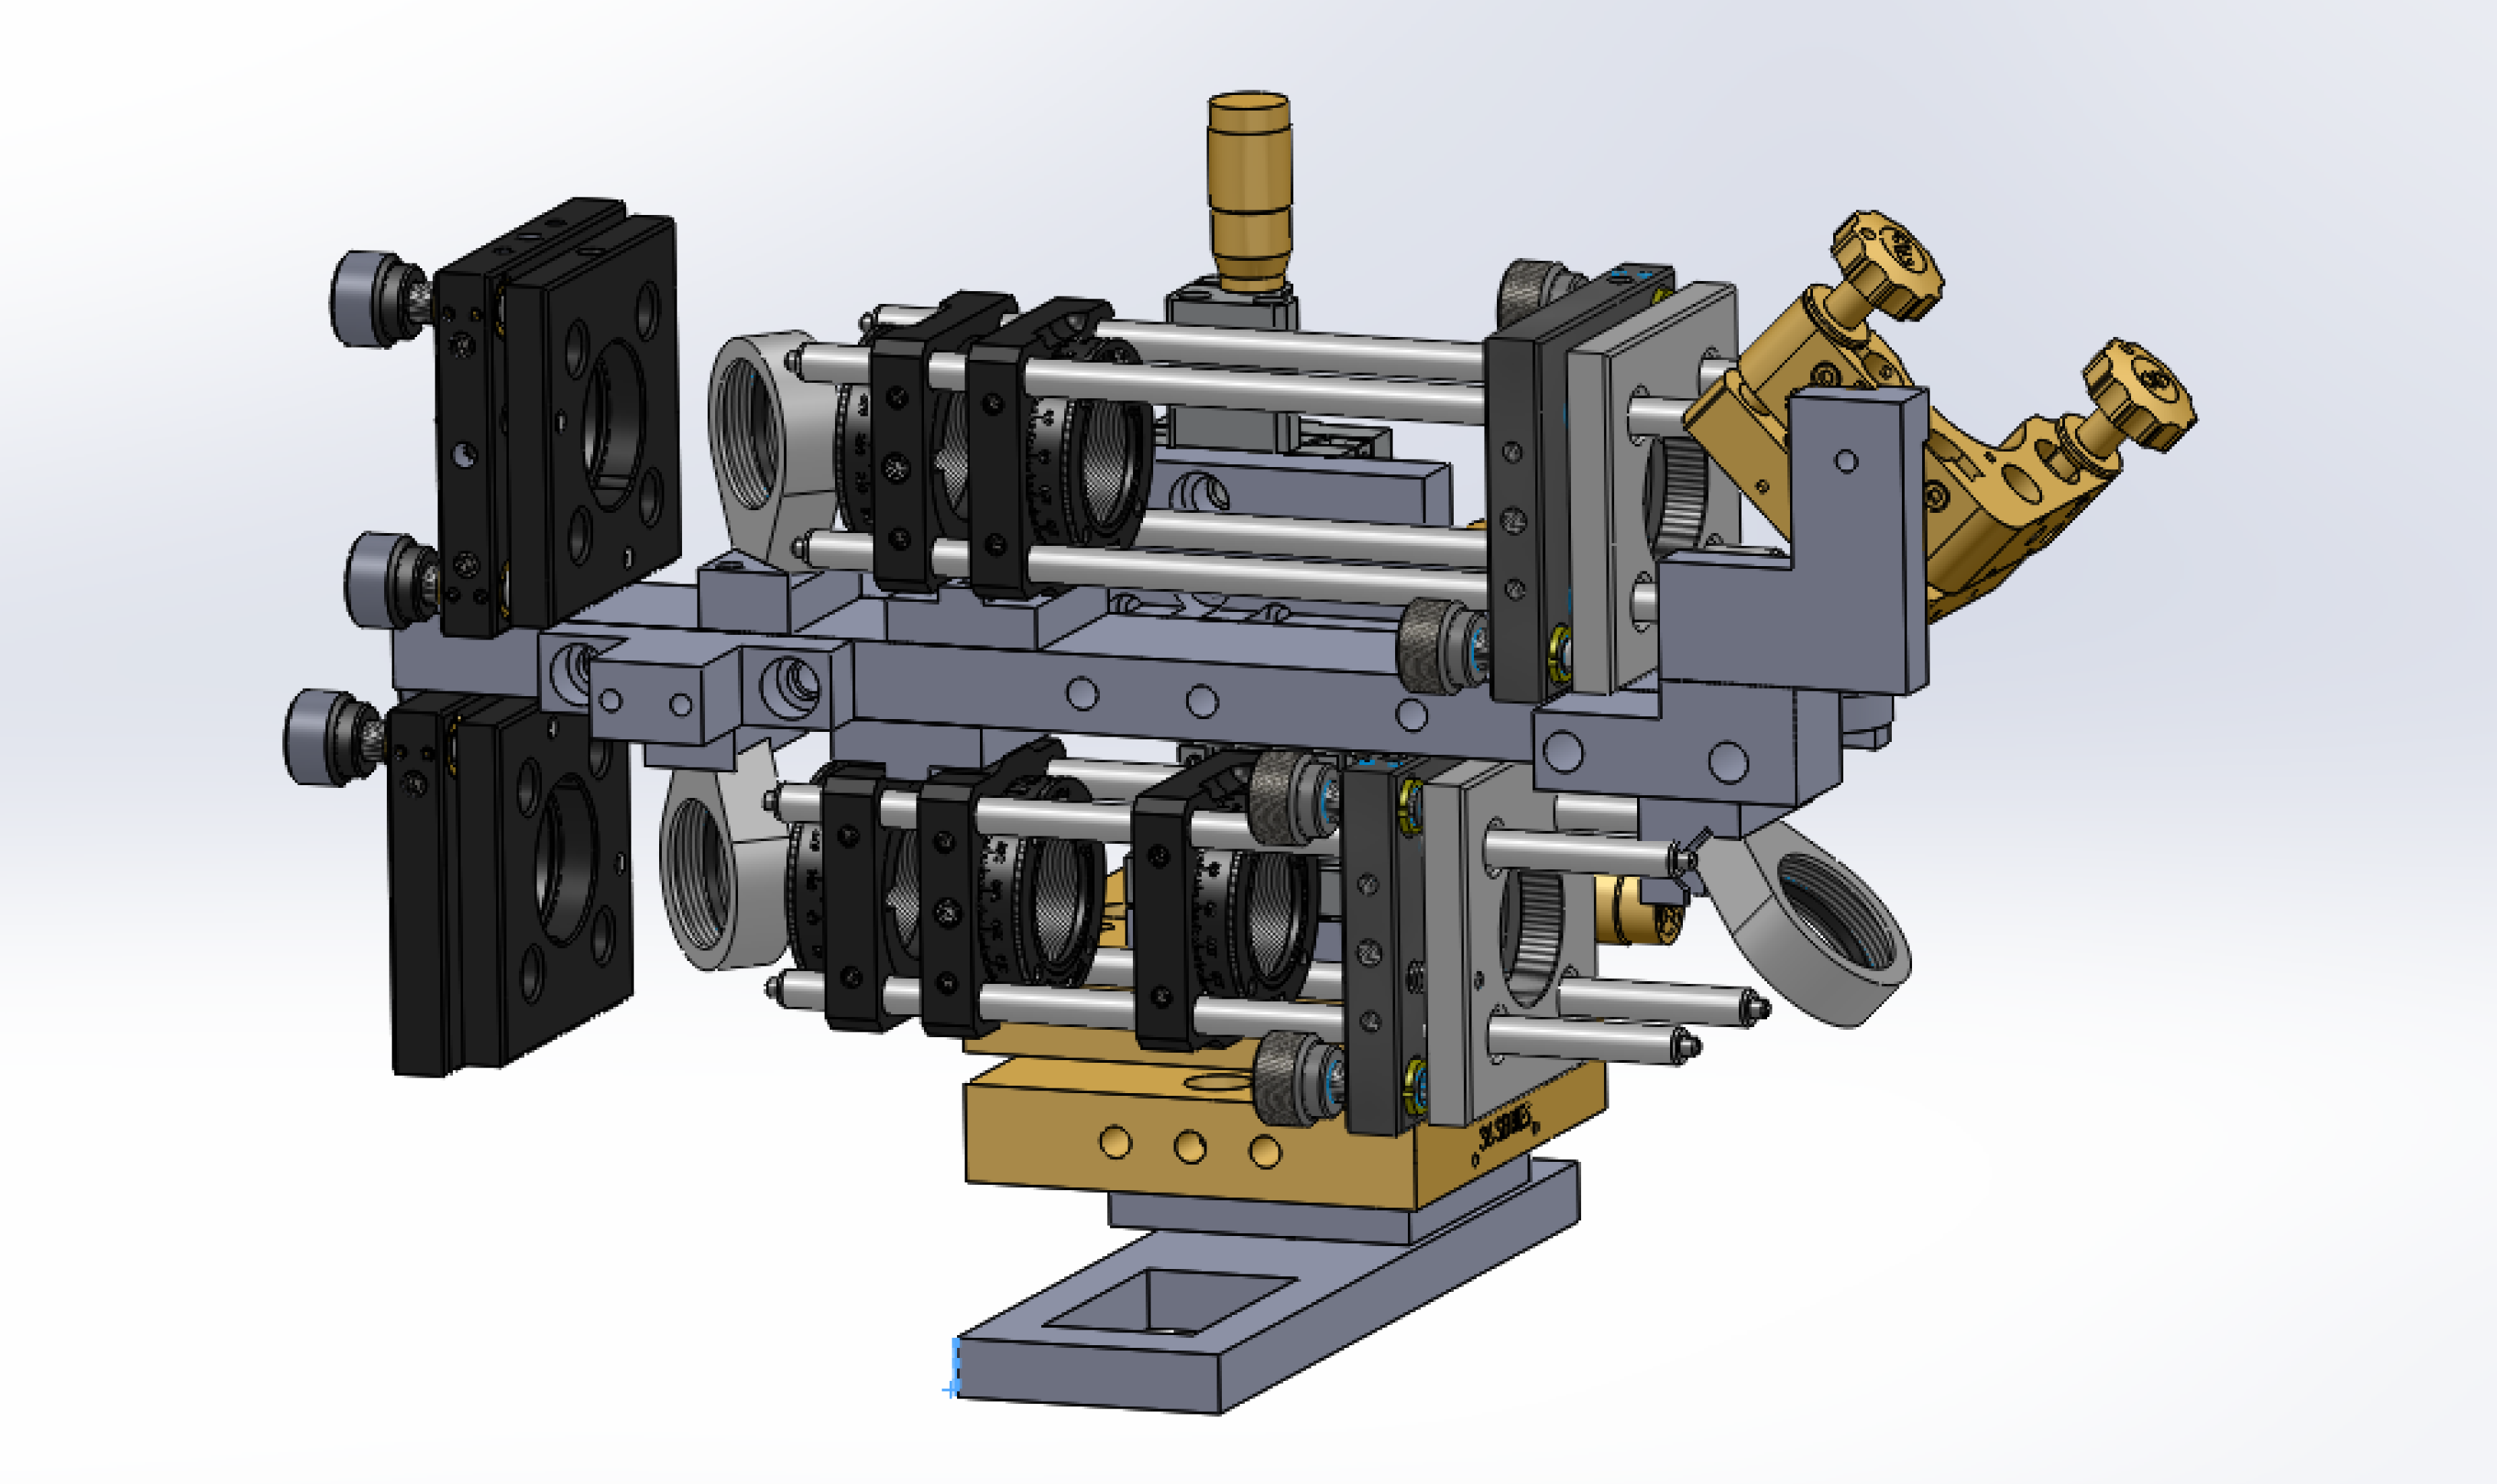
\includegraphics[width=0.48\textwidth]{../figures/lattice-assm/lattice-input-assembly.png}
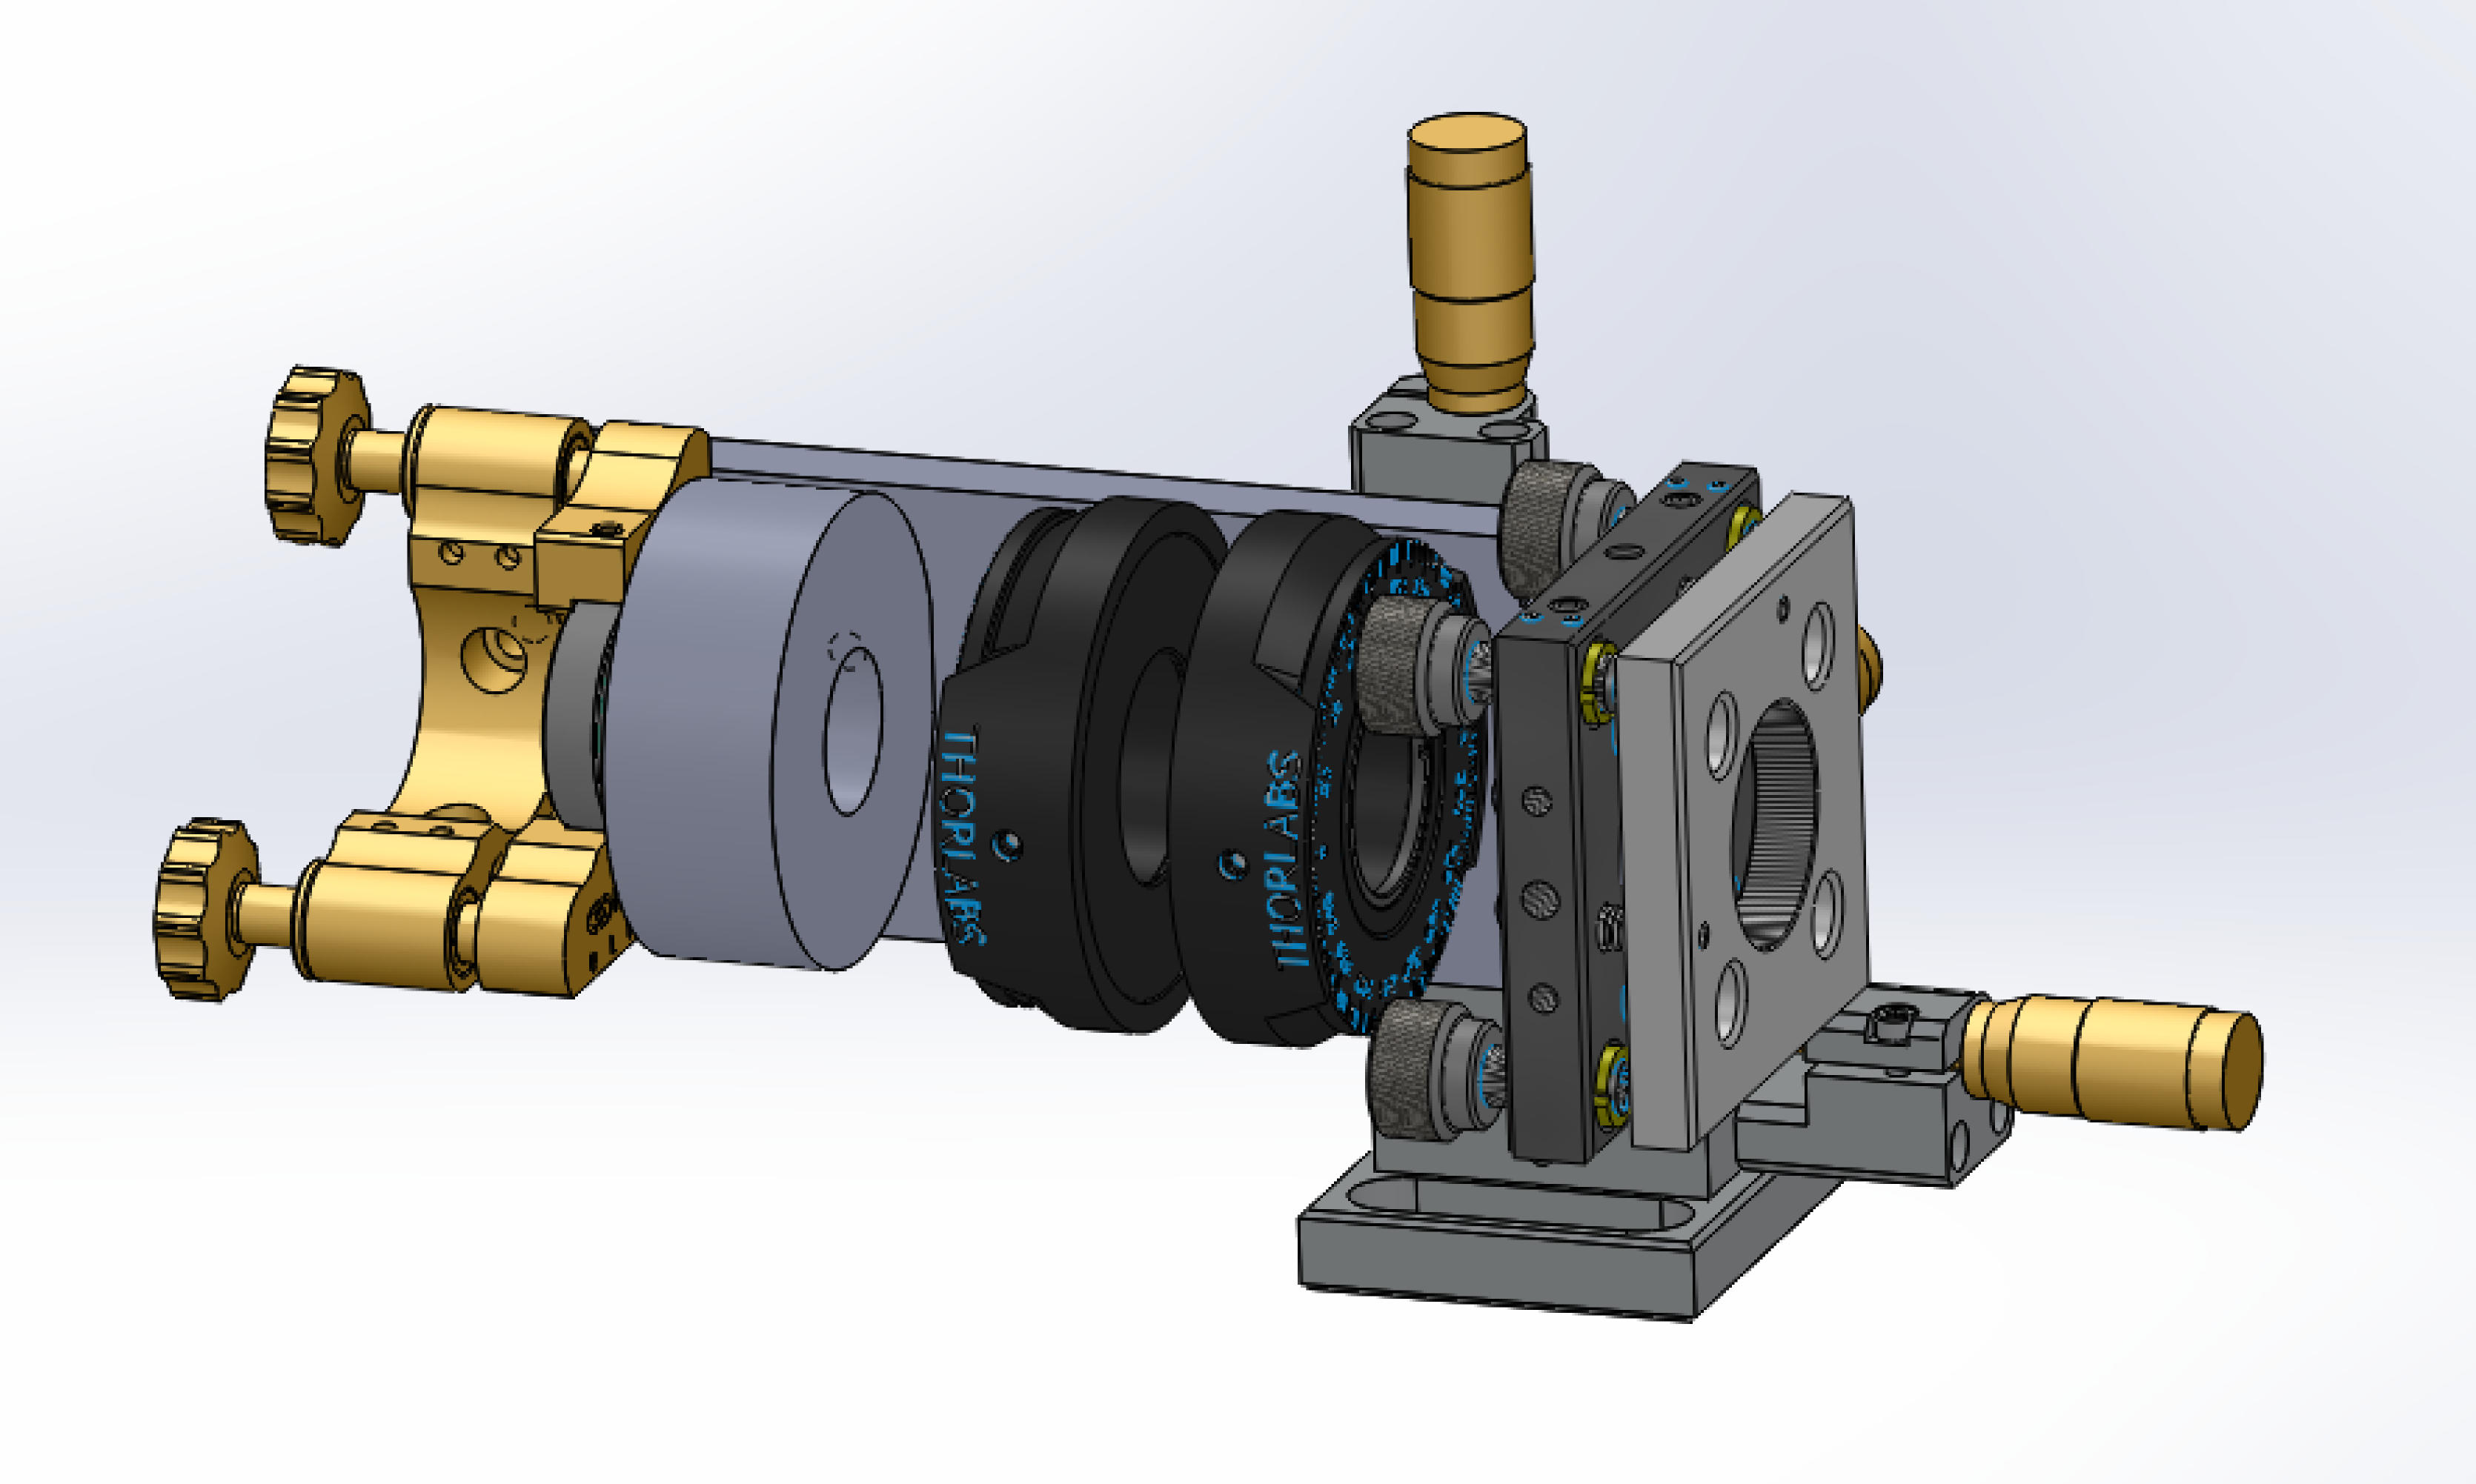
\includegraphics[width=0.48\textwidth]{../figures/lattice-assm/lattice-retro-assembly.png}
\caption{\small Input assembly for the compensated lattice (left).  Retro
assembly for the compensated lattice (right).  Refer to
Fig.~\ref{fig:comp-latt-schem} for a schematic of the optical setup in each
assembly.}
\label{fig:input-stage}
\end{figure}
\begin{figure}
    \centering
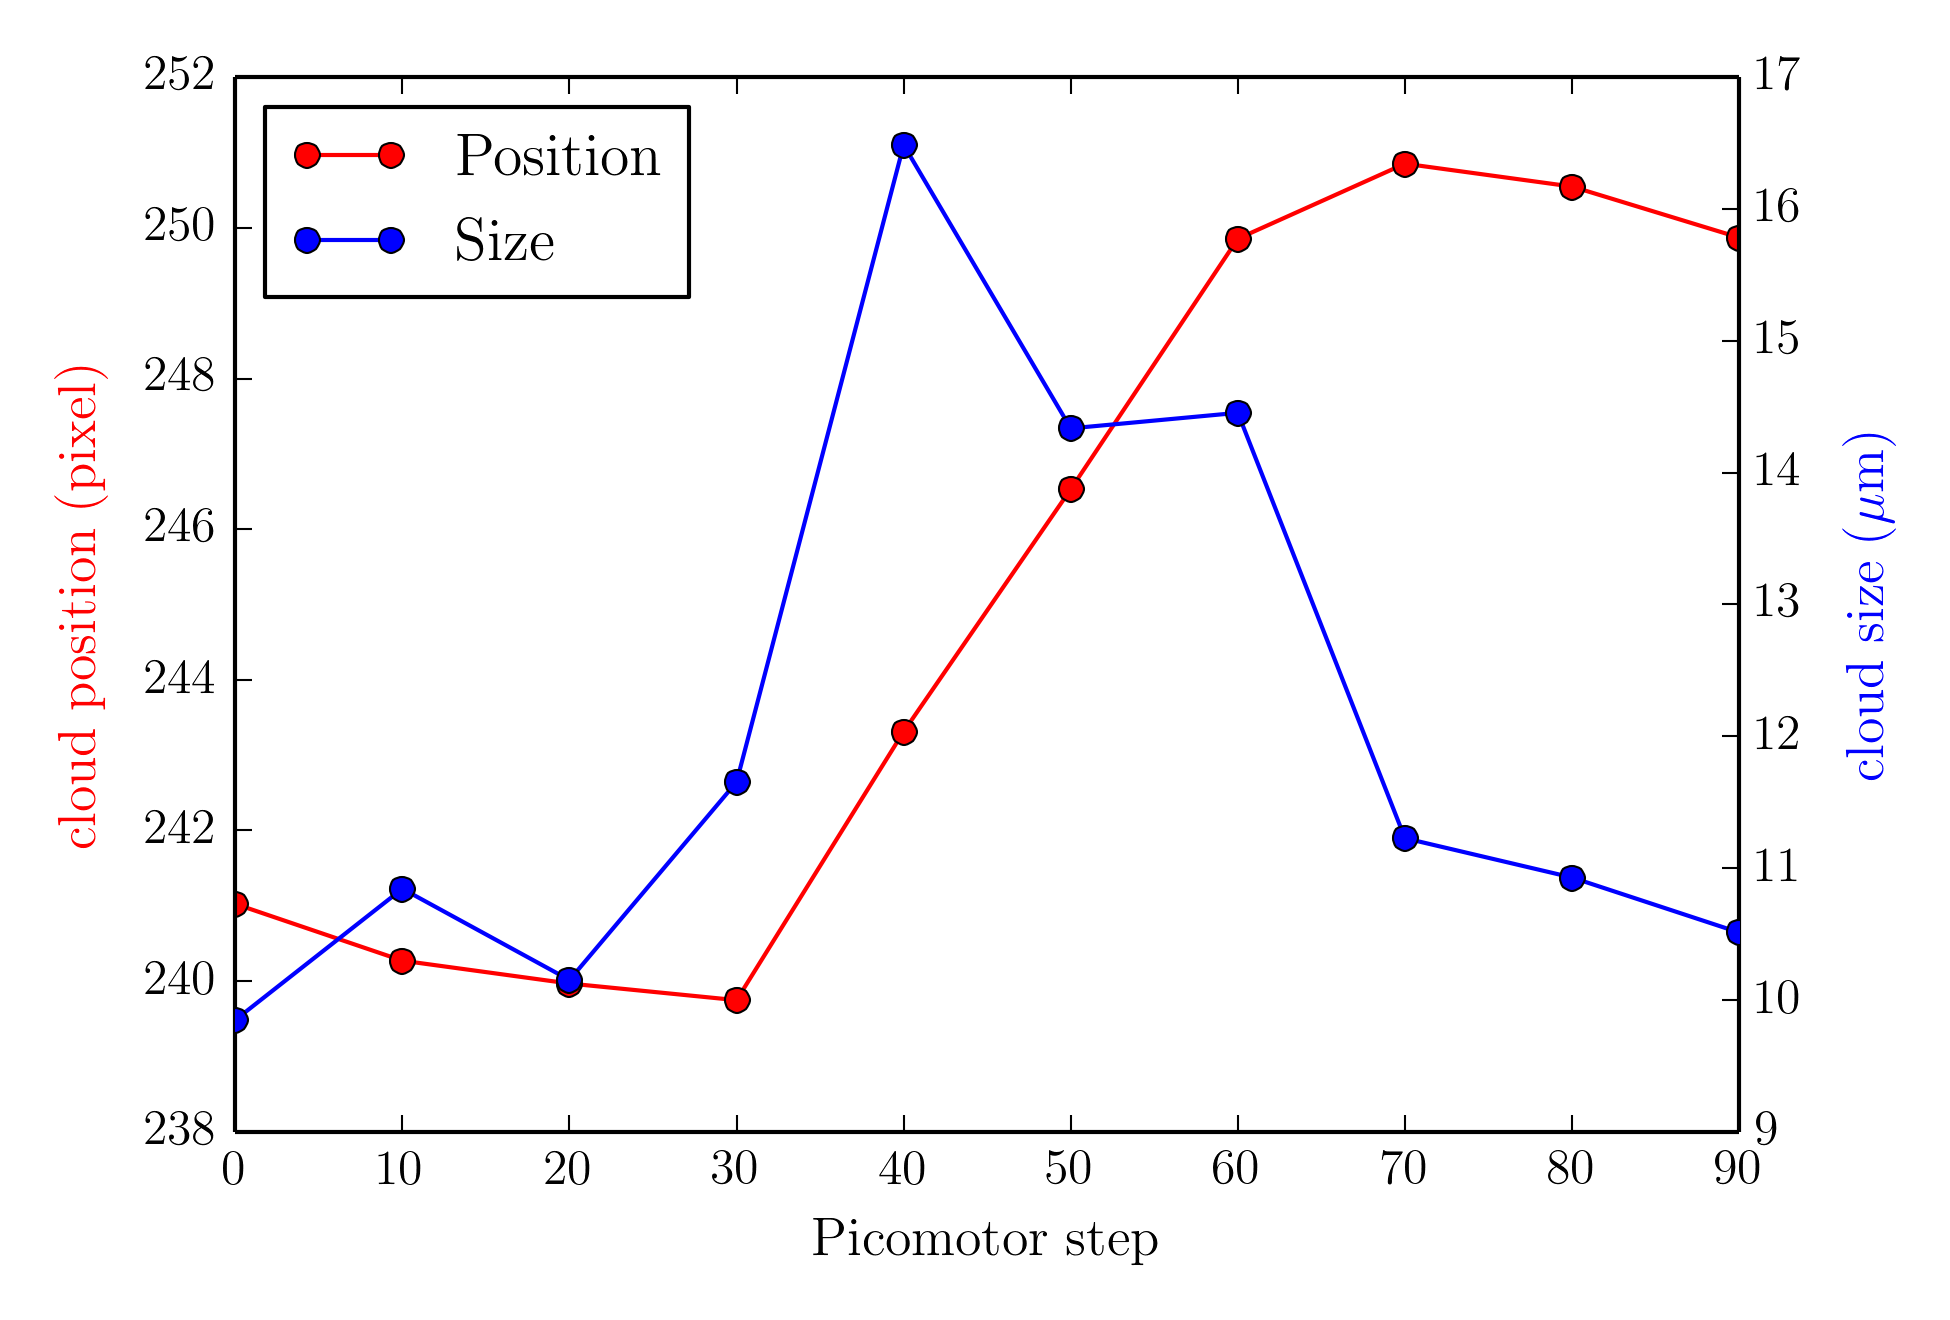
\includegraphics[width=0.58\textwidth]{../ernie-figures/lattice/overlap/pico.png}
\caption{\small Positioning of the compensation beam with PicoMotor stepper.
The position and size of the cloud in a cross beam trap of beams 1  and 3 is
plotted versus the PicoMotor actuator step. }
\label{fig:movepico}
\end{figure}

\section{Lattice loading ramps}

Once we have a cold sample in the dimple, we proceed to load it into the
optical lattice and to set the on-site interactions, $U/t$, to the desired
value for the experiment.  The ramps we have chosen to do that are piece-wise
linear in the power of the beams and in the scattering length.  Different
segments can be easily added from the control interface to tailor the ramps.
Figure~\ref{fig:lattice-load} shows the present version of the ramps, used for
the data presented in the next two chapters. 
\begin{figure}
    \centering
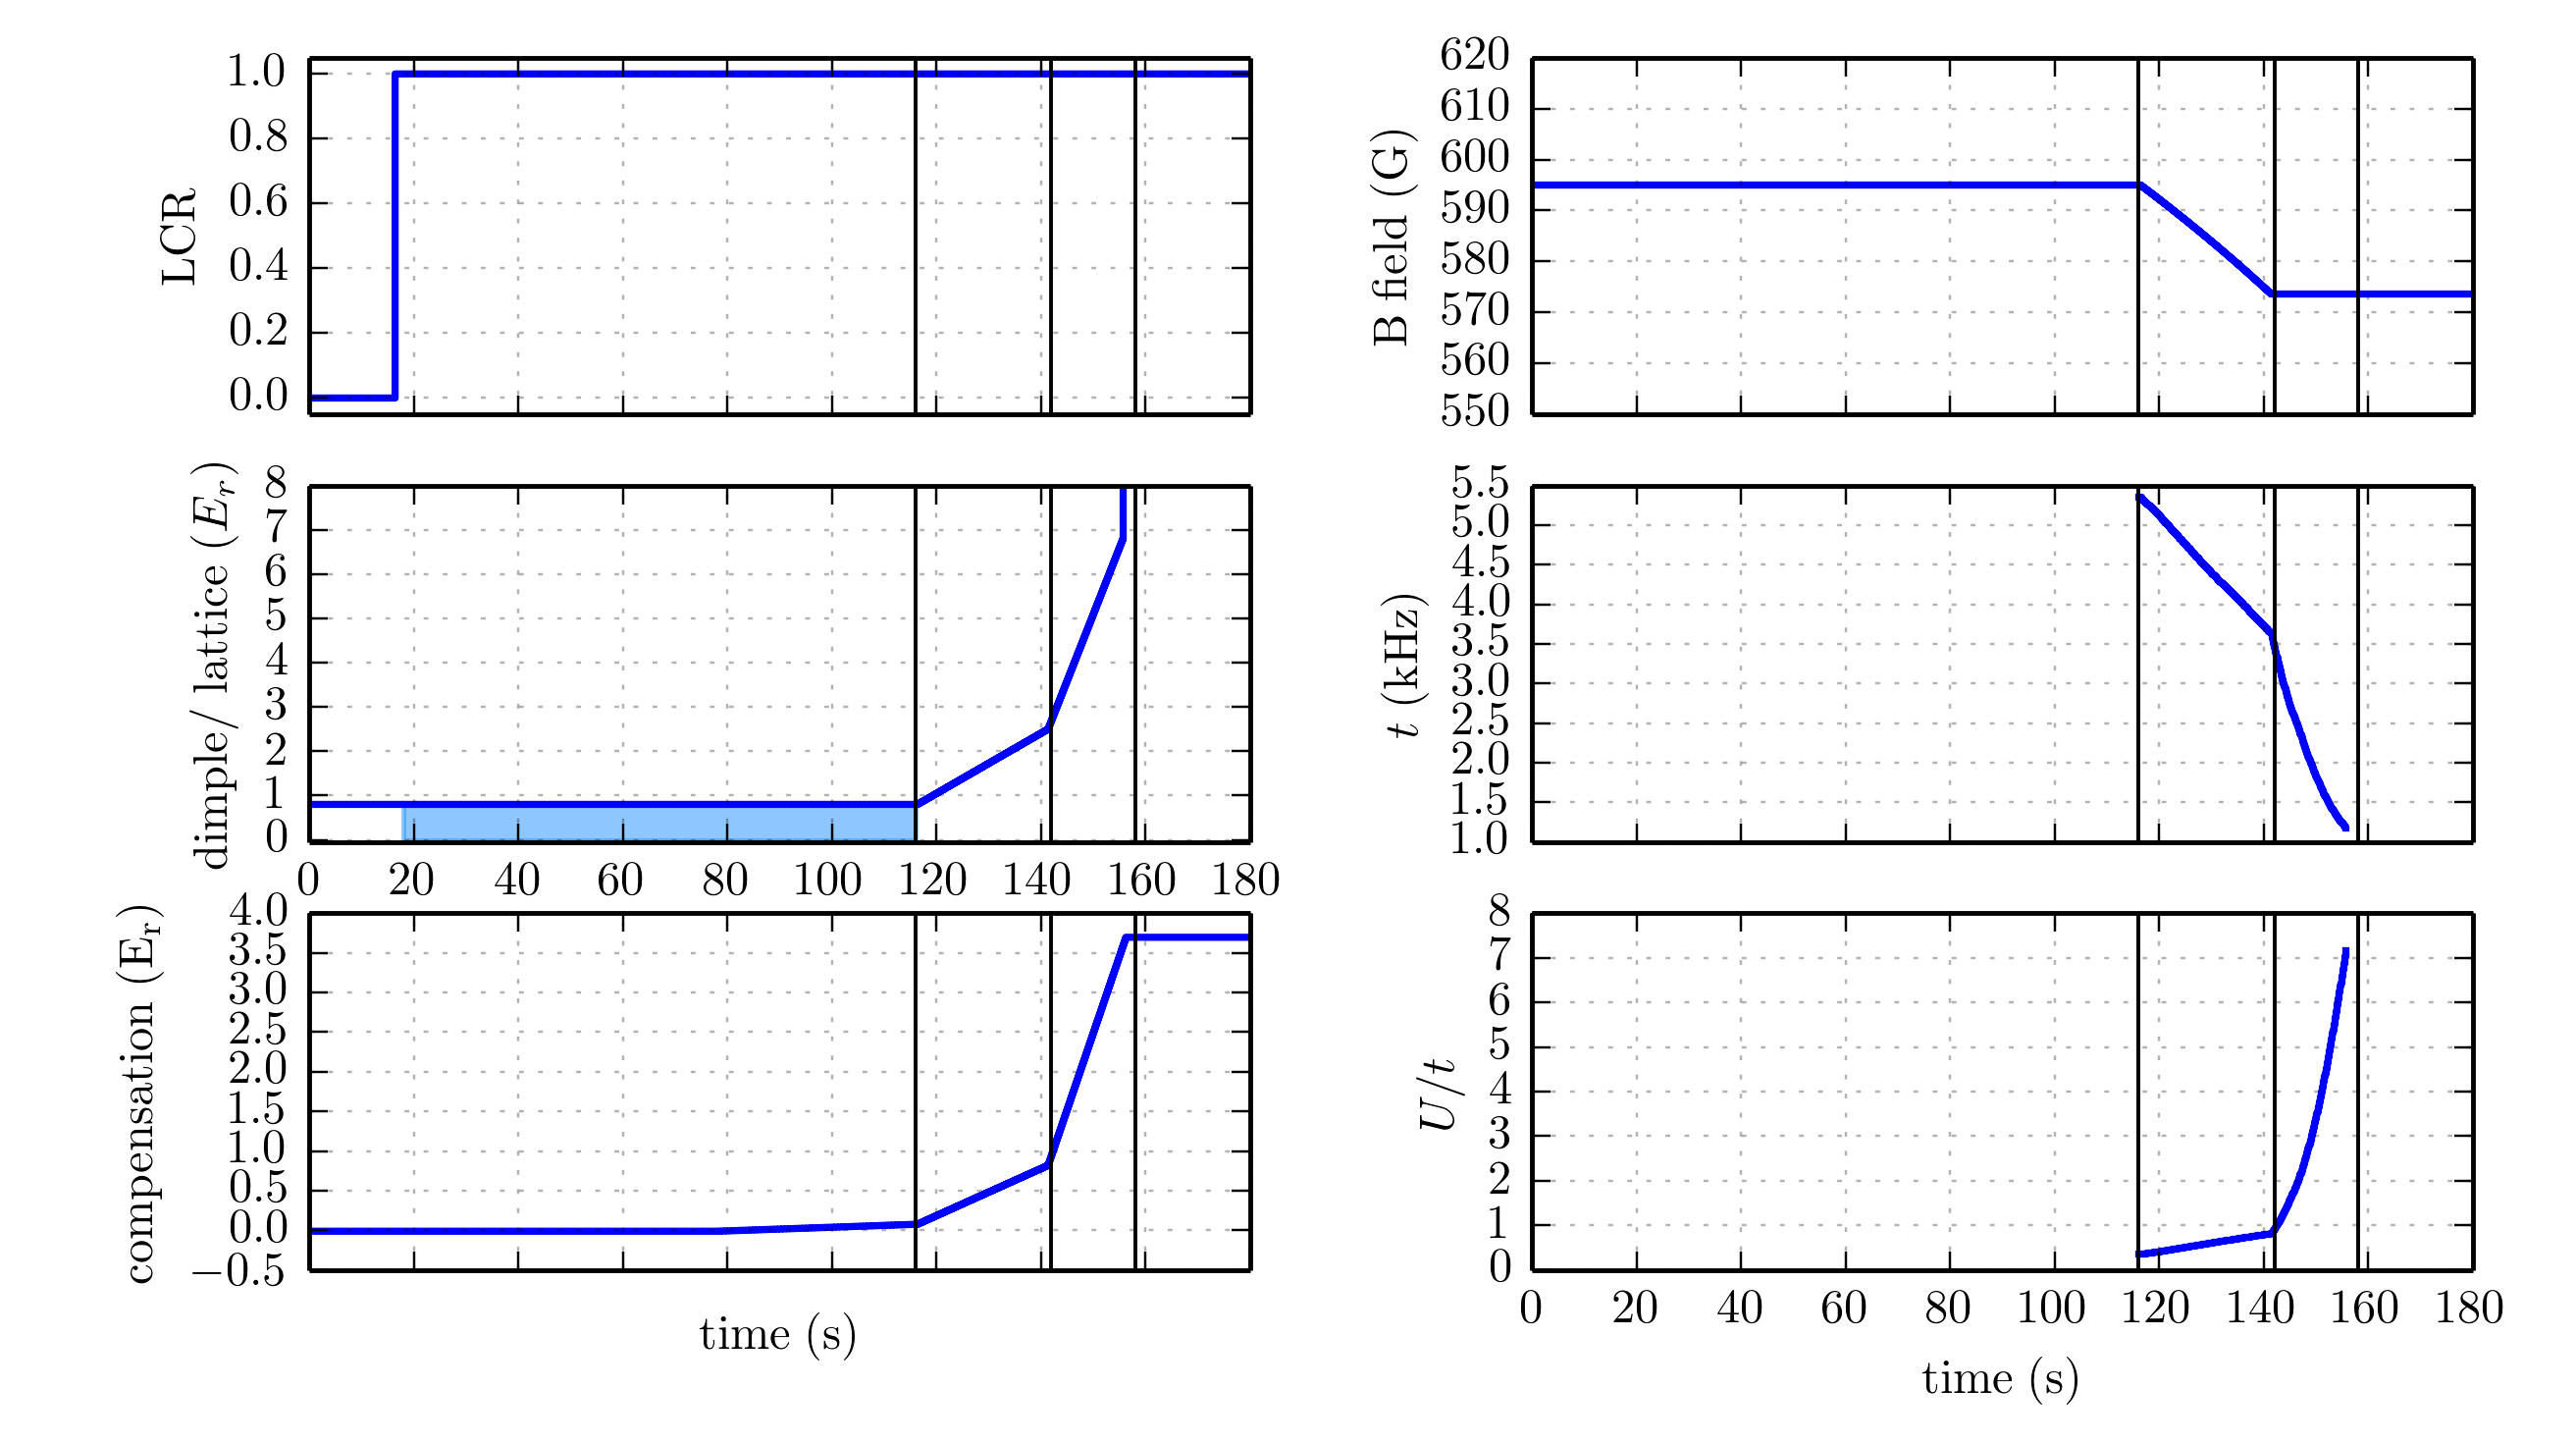
\includegraphics[width=\textwidth]{../figures/evap/load_ramp.png}
\caption{\small Lattice loading ramps.  The LCR is switched from dimple (0) to
lattice (1) mode.  By $t=116\,$ms, the polarization has fully rotated.   The
panel labeled lattice depth shows a line proportional to the power in the
lattice beams.  In dimple configuration the $y$-axis of this panel corresponds
to the the depth of the dimple trap. The depth of the dimple trap is equal to
two times the depth per axis, since the dimple trap is a three axis cross beam.
In lattice configuration the $y$-axis corresponds to the lattice depth.  The
shaded region in this plot indicates times where the retro polarization is not
fully in dimple or lattice mode.  The tunneling rate, $t$, and Hubbard
interaction $U/t$ are shown only for times where the potential is in full
lattice mode.    }
\label{fig:lattice-load}
\end{figure}

The first thing we do, is abruptly switch the control voltage to the liquid
crystal retarders (LCRs) that set the polarization of the lattice retro beams.
The response time scale ($\sim100~$ms) of the LCRs sets the time scale for the
rotation of the polarization.   We have observed that perhaps the ramps could
proceed a little faster, but we are ultimately limited by the response time of
the LCRs.

As the polarization is rotated, the sample tends to increase in density due to
the larger confinement of the lattice as compared to the dimple.  The power of
the compensation beams is increased very slightly, to keep the peak density of
the sample constant. From $t=80$ to 116~ms, 0.06\,$E_{r}$ of compensation is
added. 

After the polarization is fully rotated,  the lattice depth is increased from
0.8$\,E_{r}$ to 2.5\,$E_{r}$ in 25~ms.  This part of the lattice ramp is done
slowly  because, for lattice depths below 2.4\,$E_{r}$ the lowest and first
bands in the 3D lattice have not fully separated yet (refer to
Fig.~\ref{fig:bands3d_V0}).  During the same 25~ms the compensation is
increased to 0.65\,$E_{r}$, and also the scattering length is set (by adjusting
the magnetic field) to the value that will be used in the experiment.  

Once the 3D bands are separated, the ramps proceed more quickly and in 15~ms we
go from 2.5\,$E_{r}$ to 7\,$E_{r}$.  The compensation is adjusted to minimize
the variation of the density distribution as the ramps proceed.   At $t=156~$ms
in the figure, the lattice depth is locked to 20$\,E_{r}$ (there is no wait
time at 7\,$E_{r}$ before locking the lattice) where we proceed to measure
Bragg scattering on the \hhh\ direction.   For experiments where images of the
\textit{in-situ} density distributions are recorded we do not effect the
lattice lock.  


%\section{Round-trip temperature measurements}

